% Computing Galois Groups of Finite Fano Problems
%
% Thomas Yahl
% February 2022
%
%%%%%%%%%%%%%%%%%%%%%%%%%%%%%%%%%%%%%%%%%%%%%%%%%%%%%%%%%%%%%%%%%%%%%%%%%%%%%%%%%
\documentclass[12pt]{amsart}
\usepackage[margin = 1in]{geometry}
\usepackage{amsmath,amssymb,amsthm}
\usepackage[dvipsnames]{xcolor}
\usepackage{tikz}

%Environments
\newtheorem{theorem}{Theorem}
\newtheorem{theorem'}{Theorem*}
\newtheorem{lemma}[theorem]{Lemma}
\newtheorem{corollary}[theorem]{Corollary}
\newtheorem{proposition}[theorem]{Proposition}
\newtheorem{algorithm}[theorem]{Algorithm}

\theoremstyle{definition}
\newtheorem{definition}[theorem]{Definition}
\newtheorem{example}[theorem]{Example}
\newtheorem{remark}[theorem]{Remark}


\title{Computing Galois Groups of Finite Fano Problems}
%%%%%%%%%%%%%%%%%%%%%%%%%%%%%%%%%%%%%%%%%%%%%%%%%%%%%%%%%%%%%%%%%%%%%%%%%%%% 
\author[T.~Yahl]{Thomas Yahl} 
\address{T.~Yahl\\ 
         Department of Mathematics\\ 
         Texas A\&M University\\ 
         College Station\\ 
         Texas \ 77843\\ 
         USA} 
\email{thomasjyahl@math.tamu.edu} 
\urladdr{http://www.math.tamu.edu/~thomasjyahl} 
%%%%%%%%%%%%%%%%%%%%%%%%%%%%%%%%%%%%%%%%%%%%%%%%%%%%%%%%%%%%%%%%%%%%%%%%%%%%%%%%%%

%Macros
\newcommand{\CC}{\mathbb{C}}
\newcommand{\RR}{\mathbb{R}}
\newcommand{\ZZ}{\mathbb{Z}}
\newcommand{\gr}{\mathbb{G}}
\newcommand{\gal}{\mathcal{G}}

\newcommand{\defcolor}[1]{{\color{RoyalBlue}#1}}
\newcommand{\demph}[1]{\defcolor{{\sl #1}}}
\newcommand{\red}[1]{{\color{Red}(#1)}}

%%%%%%%%%%%%%
%%Beginning%%
%%%%%%%%%%%%%
\begin{document}

%%%%%%%%%%%%
%%Abstract%%
%%%%%%%%%%%%
\begin{abstract}
A Fano problem consists of enumerating linear spaces of a fixed dimension on a variety, generalizing the classical problem of 27 lines on a cubic surface. Those Fano problems with finitely many linear spaces have an associated Galois group that acts on these linear spaces and controls the complexity of computing them in coordinates via radicals. Galois groups of Fano problems were first studied by Jordan, who considered the Galois group of the problem of 27 lines on a cubic surface. Recently, Hashimoto and Kadets nearly classified all Galois groups of Fano problems by determining them in a special case and by showing that all other Fano problems have Galois group containing the alternating group. We use computational tools to prove that several Fano problems of moderate size have Galois group equal to the symmetric group, each of which were previously unknown.
\end{abstract}
%%%%%%%%%%%%%%%%%%%%%%%%%%%%%%%%%%%%%%%%%%%%%%%%%%%%%%%%%%%%%%%%%%%%%%%%%%%%%%%%%



\maketitle

%%%%%%%%%%%%%%%%
%%Introduction%%
%%%%%%%%%%%%%%%%
\section{Introduction}
The classical problem of 27 lines on a smooth cubic surface in $\mathbb{P}^3$ is one of the first examples of a Fano problem: enumerating $r$--planes lying on a variety $X$. The family of $r$--planes on $X$ is a subscheme of the Grassmanian called the Fano scheme of $X$. Debarre and Manivel studied Fano schemes in the setting where $X$ is a general complete intersection and determined invariants such as the dimension and degree of its Fano scheme. We concern ourselves with those complete intersections having a finite Fano scheme, each of which belongs to a parameterized family determined by combinatorial data.

To each family of Fano problems there is an associated Galois group which acts on the Fano scheme of a general complete intersection the family. Jordan was the first to study these Galois groups in his work  ``Trait\'{e} des Substitutions et des \'{E}quations Alg\'{e}briques" in which he noted the Galois group of an enumerative problem must preserve intrinsic structure of the problem \cite{Jordan}. For instance, the Galois group of the problem of lines on a cubic surface must preserve the incidence structure of these lines. From this Jordan observed this Galois group is a subgroup of the Coxeter group $E_6$.

Harris observed that the algebraic Galois groups Jordan defined are geometric monodromy groups, an idea tracing back to Hermite \cite{Hermite}. Using this, he generalized Jordan's work by studying the Galois group of lines in $\mathbb{P}^n$ on a hypersurface of degree $2n-3$. He was able to show Jordan's inclusion to be an equality and that for $n\ge 4$ this Galois group is the symmetric group on its Fano scheme---such a Galois group is called fully symmetric. To show this, Harris first showed these Galois groups are two--transitive, then showed the existence of a simple transposition in the Galois group by an explicit construction of a system satisfying certain properties.

Much of the study of Galois groups of Fano problems then laid dormant until Hashimoto and Kadets nearly determined them in all cases \cite{HK}. First, the Fano problem of $r$--planes in $\mathbb{P}^{2r+2}$ on the intersection of two quadrics was shown to have Galois group equal to the Coxeter group $D_{2r+3}$ for $r\ge 1$. Then it was shown that these Fano problems and the problem of lines on a cubic surface were unique in that all other Fano problems have Galois group containing the alternating group.

By the results of Hashimoto and Kadets, the open problem of classifying Galois groups of Fano problems rests on determining whether certain Fano problems have Galois group equal to the alternating group or the symmetric group. Towards this goal, we use computational tools to prove remaining Fano problems of moderate size have fully symmetric Galois group. We do so by extending Harris' method of proof to these Fano problems by exhibiting a simple transposition. This transposition is the result of producing a system satisfying certain properties and verify those properties with a mixture of exact computation and numerical certification. 

\begin{center}
\begin{figure}[h]
  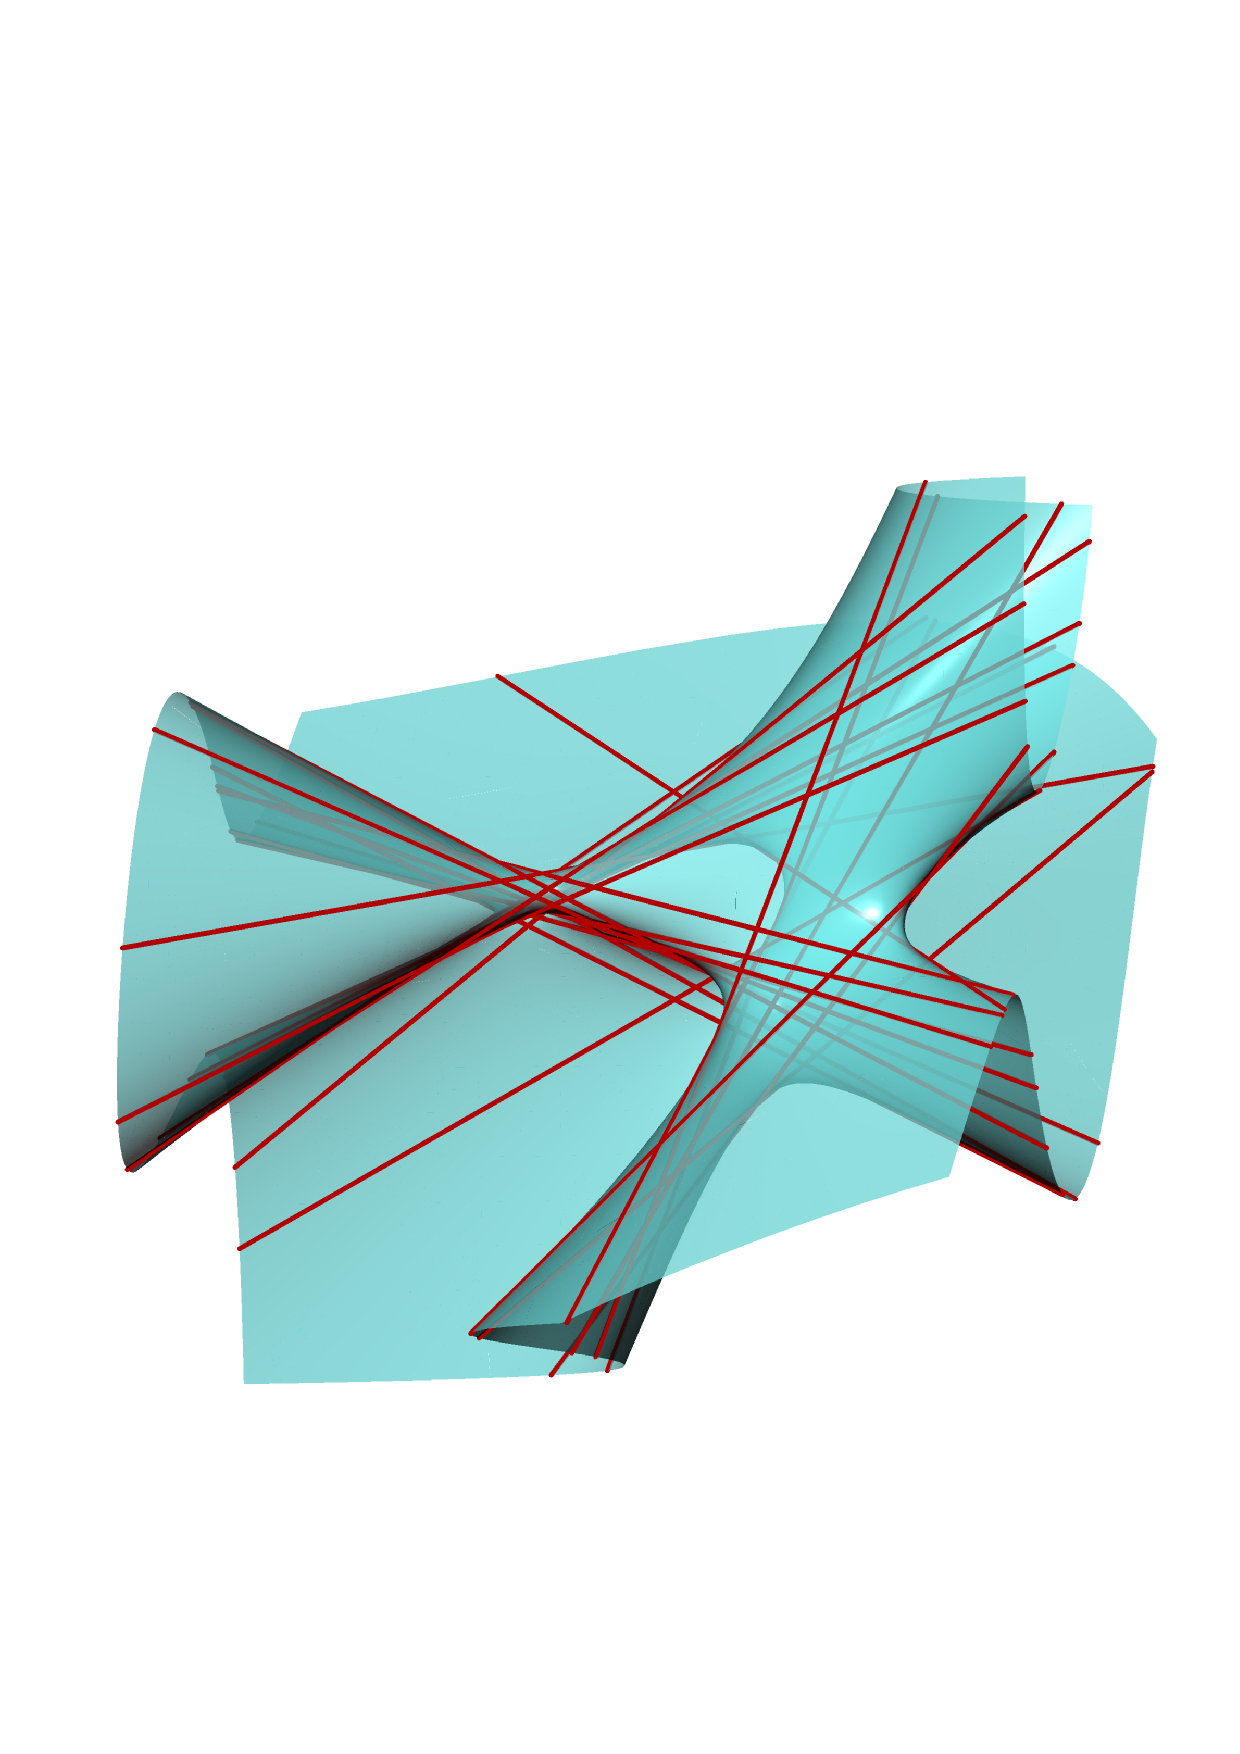
\includegraphics[scale=.38]{figures/27lines.pdf}
  \caption{27 lines on a smooth cubic surface}
\end{figure}
\end{center}



%%%%%%%%%%%%%%%%%
%%Fano Problems%%
%%%%%%%%%%%%%%%%%
\section{Fano Problems}
The family of $r$--planes in $\mathbb{P}^n$ is an irreducible projective variety known as the Grassmanian $\gr(r,\mathbb{P}^n)$ and is of dimension $(r+1)(n-r)$. For a variety $X\subseteq\mathbb{P}^n$ its \defcolor{Fano scheme} is the subscheme of $\gr(r,\mathbb{P}^n)$ of $r$--planes that lie on $X$. We study Fano schemes uniformly in the setting that $X$ is a complete intersection.

When $X\subseteq\mathbb{P}^n$ has codimension $s$, $X$ is defined by homogeneous polynomials $F = (f_1,\dotsc,f_s)$ in $n+1$ variables. Write $d_\bullet = (d_1,\dotsc,d_s)$ for the sequence of respective degrees of these polynomials, $\deg f_i = d_i$. We make the assumption that $d_i\ge 2$ for each $i$, since otherwise some $f_i$ is linear from which we may consider $X\subseteq\mathbb{P}^{n-1}$. When $X$ is smooth it contains no $r$--planes of dimension $r>\frac{1}{2}\dim X$, so we require that $2r\le n-s$.

Let $\mathbb{C}^{(r,n,d_\bullet)}$ denote the parameter space of systems of homogeneous polynomials $F = (f_1,\dotsc,f_s)$ in $n+1$ variables of respective degrees $d_\bullet = (d_1,\dotsc,d_s)$. For general $F\in\mathbb{C}^{(r,n,d_\bullet)}$ the zero set $\mathcal{V}(F)$ is a smooth complete intersection whose Fano scheme of $r$--planes we denote by $\mathcal{V}_r(F)$. The combinatorial data $(r,n,d_\bullet)$ is the \defcolor{type} of the Fano scheme $\mathcal{V}_r(F)$ and we say this Fano scheme is general if $F\in\mathbb{C}^{(r,n,d_\bullet)}$ is general. We wish to understand for which data $(r,n,d_\bullet)$ a general Fano scheme of type $(r,n,d_\bullet)$ is zero-dimensional. 


%Dimension & degree
Fix $F = (f_1,\dotsc,f_s)\in\mathbb{C}^{(r,n,d_\bullet)}$. We note that $\ell\in\mathcal{V}_r(F)$ exactly when $F|_\ell = 0$. Each $f_i$ restricts to a degree $d_i$ form on $\ell$ whose vanishing amounts to the vanishing of its $\left(\begin{smallmatrix}r+d_i\\r\end{smallmatrix}\right)$ coefficients. Since $\gr(r,\mathbb{P}^n)$ has dimension $(r+1)(n-r)$, the expected dimension of the Fano scheme $\mathcal{V}_r(F)$ is given by 
\begin{align*}
\delta(r,n,d_\bullet) = (r+1)(n-r) - \sum_{i=1}^s\begin{pmatrix}r+d_i\\d_i\end{pmatrix}.
\end{align*}
Debarre and Manivel \cite{DM} showed that this expected dimension is the dimension in general.

\begin{theorem}[Debarre,Manivel]
The general Fano scheme of type $(r,n,d_\bullet)$ has dimension $\delta(r,n,d_\bullet)$ when $\delta(r,n,d_\bullet)\ge 0$ and is empty otherwise.
\end{theorem}

We say the \defcolor{Fano problem} $(r,n,d_\bullet)$ is the problem of describing a general Fano scheme of type $(r,n,d_\bullet)$, where $\delta(r,n,d_\bullet)=0$. That is, a Fano problem is that of describing a finite general Fano scheme.

Since the Grassmanian is a projective variety, a Fano scheme has a well-defined degree. By expressing a Fano scheme of type $(r,n,d_\bullet)$ as a chern class of a vector bundle on $\mathbb{G}(r,\mathbb{P}^n)$, the splitting lemma can be used to write this degree explicitly. Debarre and Manivel gave a general formula.

Define the quantities
\begin{align*}
Q_{r,d}(x) = \prod_{\stackrel{a_i\in\mathbb{Z}_{\ge 0}}{a_0+\dotsb+a_r=d}}(a_0x_0 + \dotsb + a_rx_r)\in\mathbb{Z}[x_0,\dotsb,x_r]
\end{align*}
and $Q_{r,d_\bullet}(x) = Q_{r,d_0}(x)\dotsb Q_{r,d_s}(x)$, as well as the Vandermonde polynomial
\begin{align*}
V_r(x) = \prod_{0\le i<j\le r}(x_i-x_j).
\end{align*}

\begin{theorem}[Debarre,Manivel]
If $(r,n,d_\bullet)$ is a Fano problem, the degree of a general Fano scheme of type $(r,n,d_\bullet)$, $\deg(r,n,d_\bullet)$, is equal to the coefficient of $x_0^n x_1^{n-1}\dotsb x_r^{n-r}$ in the product $Q_{r,d_\bullet}(x)V_r(x)$.
\end{theorem}

Table \ref{Small Fano} shows some Fano problems of small degree. 

\begin{table}[htb]
  \caption{Small Fano problems}
  \label{Small Fano}
  \def\arraystretch{1.2}
  \begin{tabular}{||c|c|c|c|c||}
    \hline
    $~r~$ & $~n~$ & $~d_\bullet~$ & $~\deg(r,n,d_\bullet)~$ & ~Galois Group~\\
    \hline\hline
    1 & 4 & $(2,2)$ & 16 & $D_5$\\
    \hline
    1 & 3 & $(3)$ & 27 & $E_6$\\
    \hline
    2 & 6 & $(2,2)$ & 64 & $D_7$\\
    \hline
    3 & 8 & $(2,2)$ & 256 & $D_9$\\
    \hline
    1 & 7 & $(2,2,2,2)$ & 512 & $S_{512}$\\
    \hline
    1 & 6 & $(2,2,3)$ & 720  & $S_{720}$\\
    \hline
    4 & 10 & $(2,2)$ & 1024 & $D_{11}$\\
    \hline
    2 & 8 & $(2,2,2)$ & 1024  & $S_{1024}$\\
    \hline
  \end{tabular}
\end{table}

By using lower bounds on the degree of a Fano problem, those with degree less than a set amount can be enumerated. For instance, the following is a lower bound on the degree of a Fano problem that may be used.

\begin{proposition}
Let $(r,n,d_\bullet)$ be a Fano problem. We have
\begin{align*}
\deg(r,n,d_\bullet) \ge \prod_i \prod_{\stackrel{1\le j\le r+1}{j|d_i}} \left(\frac{d_i}{j}\right)^{\left(\begin{smallmatrix}r+1\\j\end{smallmatrix}\right)}.
\end{align*}
\end{proposition}
\begin{proof}
Consider the product expansion of $Q_{r,d_i}(x)$. For each $1\le j\le r+1$ such that $j|d_i$, there are $\left(\begin{smallmatrix}r+1\\j\end{smallmatrix}\right)$ many terms of the product with $j$ of the $a_k$ equal to $d_i/j$. This then factors out as a constant factor of $Q_{r,d_i}(x)$ and hence of every term of $Q_{r,d}(x)V_r(x)$.
\end{proof}



%%%%%%%%%%%%%%%%%%%%%%%%%%%%%%%%%%
%%Galois Groups of Fano Problems%%
%%%%%%%%%%%%%%%%%%%%%%%%%%%%%%%%%%
\section{Galois Groups of Fano Problems}
A Fano problem $(r,n,d_\bullet)$ determines an incidence correspondence.
\begin{center}
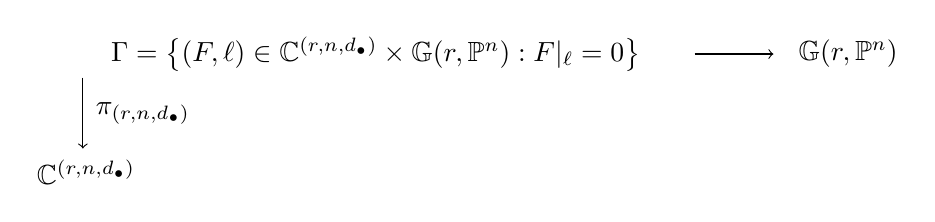
\begin{tikzpicture}
\node at (0,1.5) {$\Gamma = \left\{ (F,\ell)\in\mathbb{C}^{(r,n,d_\bullet)}\times\gr(r,\mathbb{P}^n):F|_\ell=0 \right\}$};
\draw[->] (-3.72,1.2)--(-3.72,.3) node [right] at (-3.68,.75) {$\pi_{(r,n,d_\bullet)}$};
\node at (-3.68,0) {$\mathbb{C}^{(r,n,d_\bullet)}$};
\draw[->] (4.05,1.5)--(5.05,1.5);
%\node [above] at (4.55,1.5) {$\rho$};
\node at (6,1.5) {$\mathbb{G}(r,\mathbb{P}^n)$};
\end{tikzpicture}
\end{center}
The map $\rho$ realizes the incidence variety $\Gamma$ as a vector bundle over $\mathbb{G}(r,\mathbb{P}^n)$, as the fibers are the linear spaces of systems $F\in\mathbb{C}^{(r,n,d_\bullet)}$ that vanish on a given $r$--plane. As a result, $\Gamma$ is smooth and of dimension $\dim \mathbb{C}^{(r,n,d_\bullet)}$. 

Given $F\in\mathbb{C}^{(r,n,d_\bullet)}$, the fiber $\pi_{(r,n,d_\bullet)}^{-1}(F)$ is the Fano scheme $\mathcal{V}_r(F)$. By the results of Debarre and Manivel, there is a Zariski open set $U$ with the property that if $F\in U$, the fiber $\pi_{(r,n,d_\bullet)}^{-1}(F)$ consists of $\deg(r,n,d_\bullet)$ smooth points. It follows that the restriction of $\pi_{(r,n,d_\bullet)}$ to $\pi_{(r,n,d_\bullet)}^{-1}(U)$ is a smooth covering space of degree $\deg(r,n,d_\bullet)$. 

Fix a base point $F\in U$. Every loop in $U$ based at $F$ lifts to paths in $\Gamma$ connecting points of the fiber $\pi_{(r,n,d_\bullet)}^{-1}(F)$, and the endpoints of these paths determine a permutation of this fiber. The set of all permutations obtained this way is the monodromy group of $\pi_{(r,n,d_\bullet)}$ and is defined up to isomorphism for different choices of base point $F\in U$ and reordering of the fiber $\pi_{(r,n,d_\bullet)}^{-1}(F)$. The monodromy group of $\pi_{(r,n,d_\bullet)}$ is transitive since $X$ is irreducible, while higher transitivity is equivalent to irreducibility of certain fiber products \cite{ngalois,GGEGA}. More detail about monodromy groups can be found in \cite{Hatcher}. 

\begin{definition}
The \defcolor{Galois group} of the Fano problem $(r,n,d_\bullet)$, $\gal_{(r,n,d_\bullet)}$, is the monodromy group of $\pi_{(r,n,d_\bullet)}$. 
\end{definition}

These Galois groups were first defined algebraically by Jordan \cite{Jordan}. The map $\pi:\Gamma\to\mathbb{C}^{(r,n,d_\bullet)}$ induces a reverse inclusion of the function fields of these varieties $\mathbb{C}(\mathbb{C}^{(r,n,d_\bullet)})\hookrightarrow\mathbb{C}(\Gamma)$. This expresses $\mathbb{C}(\Gamma)$ as an algebraic extension of $\mathbb{C}(\mathbb{C}^{(r,n,d_\bullet)})$ of degree $\deg(r,n,d_\bullet)$. The Galois group of the Fano problem $(r,n,d_\bullet)$ Jordan defined is the Galois group of the normal closure of this field extension. The equivalence of the geometric definition with this algebraic definition was shown by Harris \cite{Harris}, but traces back to Hermite \cite{Hermite}. 

Jordan considered the problem of lines on a cubic surface and its Galois group, $\gal_{(1,3,(3))}$. He observed that the Galois group acting on a given Fano scheme must preserve the incidence structure of the lines, and so is a subgroup of the Coxeter group $E_6$. 

Harris later proved Jordan's inclusion to be an equality, $\gal_{(1,3,(3))} = E_6$, and studied a generalization of this problem. He showed that for $n\ge 4$, the Fano problem of lines in $\mathbb{P}^n$ on a hypersurface of degree $2n-3$ is fully symmetric \cite{Harris}. To prove this, Harris observed these Galois groups are highly transitive and observed systems $F\in\mathbb{C}^{(1,n,(2n-3))}$ whose local monodromy is generated by a simple transposition.

Hashimoto and Kadets later took up the study of these Galois groups more generally. They studied the Fano problem of $r$--planes in $\mathbb{P}^{2r+2}$ on the intersection of two quadrics and determined the Galois group to be the Coxeter group $\gal_{(r,2r+2,(2,2))} = D_{2r+3}$. It was then showed that when $d_\bullet\ne(3),(2,2)$, the $r$--planes do not intersect for a general Fano scheme of type $(r,n,d_\bullet)$. As a result of this, $\gal_{(r,n,d_\bullet)}$ is highly transitive and contains the alternating group on its solutions when $d_\bullet\ne(3),(2,2)$ \cite{HK}.



%%%%%%%%%%%%%%%%%%%%%%%%%
%%Computational Methods%%
%%%%%%%%%%%%%%%%%%%%%%%%%
\section{Computational Methods}
Harris exhibited a simple transposition in the Galois groups $\gal_{(1,n,(2n-3))}$ by producing systems $F\in\mathbb{C}^{(1,n,(2n-3))}$ with the property that the fiber $\pi_{(1,n,(2n-3))}^{-1}(F)=\mathcal{V}_r(F)$ has degree $\deg(1,n,(2n-3))$, contains a unique double point, and is otherwise smooth. The local monodromy around such a point generates a simple transposition \cite{Harris}. 

To be able to extend this technique of Harris to a Fano problem $(r,n,d_\bullet)$, we must be able to verify the fiber $\pi_{(r,n,d_\bullet)}^{-1}(F)$ over $F\in\mathbb{C}^{(r,n,d_\bullet)}$ contains a double point and that there are $\deg(r,n,d_\bullet)-2$ smooth points. For $F\in\mathbb{C}^{(r,n,d_\bullet)}$, the fiber $\pi_{(r,n,d_\bullet)}^{-1}(F)$ can be expressed as zeros of a polynomial system after choosing appropriate coordinates on $\mathbb{G}(r,\mathbb{P}^n)$. This allows for the use of symbolic and numerical techniques to verify our claims. 

To show our systems have the correct number of smooth zeros, we use numerical certification to isolate smooth solutions into disjoint sets. We demonstrate two distinct flavors of numerical certification, that of Smale's $\alpha$--theory and interval arithmetic. We let $G$ be a square system of $m$ polynomials and $m$ variables, and $x\in\mathbb{C}^m$.

%alpha--theory
\subsection*{$\alpha$--Theory}
Smale's $\alpha$--theory starts by defining three quantities $\alpha(G,x)$, $\beta(G,x)$, and $\gamma(G,x)$ to a system $G$ and a point $x$. The first quantity is the product $\alpha(G,x) = \beta(G,x)\gamma(G,x)$, where $\beta(G,x)$ is the step size of the Newton operator of $G$ applied to $x$ and $\gamma(G,x)$ is a measure of the size of the derivatives of $G$ at $x$. These quantities are used to isolate smooth zeros of $G$ as follows \cite{SmaleShub}.

\begin{theorem}
If $G$ is a square polynomial system in $m$ variables and $x\in\mathbb{C}^m$ is such that
\begin{align*}
\alpha(G,x) < \frac{13-3\sqrt{17}}{4} \approx .15767,
\end{align*}
then $x$ converges under iterations of the Newton operator to a zero of $G$, $\zeta\in\mathbb{C}^m$. Further, $||x-\zeta||<2\beta(G,x)$. 
\end{theorem}

The full strength of Smale's $\alpha$--theory is not seen above, as it guarantees that $x$ converges rapidly to $\zeta$ and gives a rate of convergence. This may also be used to certify all points in a neighborhood of $x$ converge to $\zeta$ under Newton's method and certify real zeros of polynomial systems. Softwares such as \texttt{alphaCertified} \cite{alphaCertified} use bounds on $\alpha(G,x)$ and similar results to enumerate and isolate zeros of polynomial systems given approximate zeros. 

When $\alpha(G,x)<\frac{1}{4}(13-3\sqrt{17})$, we obtain a bounding ball of a zero of $G$ centered at $x$ and with radius $2\beta(G,x)$. If the coefficients of $G$ and the coordinates of $x$ are given by complex rational numbers, we can use exact computation to test membership for this open ball or whether two or more of these balls are disjoint. These disjoint bounding balls will allow us to certify zeros of our system are smooth, as we will soon see.

%Interval arithmetic
\subsection*{Interval Arithmetic}
A more lax approach to numerical certification comes from interval arithmetic. A complex interval is a set of complex numbers whose real and imaginary parts lie in a pair of given intervals. The setwise sum and difference of two complex intervals is a complex interval, however the setwise product of two complex intervals need not be. Usual arithmetic operations are defined on the space of complex intervals as to contain their setwise counterpart. This allows for the evaluation of polynomials and other functions at complex intervals, the result of which contains the setwise evaluation of the function. More information on complex intervals and their arithmetic can be found in \cite{Mayer}.

The Krawczyk operator of $G$ given a point $x$ and an invertible $m\times m$ matrix $Y$, $K_{G,x,Y}$, is a generalization of the Newton operator that acts on the space of complex intervals. A result due to Rump allows us isolate zeros to $G$ using the Krawczyk operator \cite{Rump}. Older versions of this theorem exist for real intervals, and more refined theorems exist for complex intervals.

\begin{theorem}[Rump]
Let $G$ be a square polynomial system in $m$ variables, $x\in\mathbb{C}^m$ a point, and $Y$ an invertible $m\times m$ matrix. If $I$ is a complex interval such that
\begin{align*}
K_{G,x,Y}(I)\subseteq I,
\end{align*}
then $I$ contains a zero of $G$.
\end{theorem}

As was the case above, interval arithmetic allows one to compute bounding sets on zeros of a system $G$. These bounding sets will serve the same purpose--in certifying zeros to our system are smooth. The benefit of using interval arithmetic is that the condition above can be certified with floating-point arithmetic and proper rounding etiquitte. This computational ease drastically decreases the time required to compute and certify bounding sets for zeros of a system \cite{BRT}.

Numerical certification using inverval arithmetic has been implemented in the \texttt{julia} package \texttt{HomotopyContinuation.jl} \cite{HCJL}. Given a system $G$ and an approximate zero $x$, this package will provide an interval satisfying the condition above if one can be found. 

%simple double roots
\subsection*{Simple Double Roots}
Let $G$ be a square polynomial system and denote its Jacobian and Hessian by $DG$ and $D^2G$ respectively. A point $x\in\mathbb{C}^m$ is a \defcolor{simple double zero} of $G$ if $G(x)=0$, $\ker DG(x)$ is spanned by a single non-zero vector $v\in\mathbb{C}^m$, and
\begin{align*}
D^2G(x)(v,v)\not\in\text{Im}\,DG(x).
\end{align*}
Dedieu and Shub studied simple double zeros of square polynomial systems in efforts to extend Smale's $\alpha$--theory. In their work, they compute a positive separation bound for simple double zeros of a system from other zeros of the same system, showing that simple double zeros are isolated zeros of multiplicity two in the process. 

We choose our system in a such a way that $G$, $x$, and $v$ will be given by complex rational numbers. In this case, the above is a symbolic computation. That is, we can say exactly whether $x$ is a simple double root of $G$.



%%%%%%%%%%%
%%Results%%
%%%%%%%%%%%
\section{Results}
Let $(r,n,d_\bullet)$ be a Fano problem with $d_\bullet\ne(3),(2,2)$. As a means of finding $F\in\mathbb{C}^{(r,n,d_\bullet)}$ with the desired properties, we prescribe a subscheme of $\mathcal{V}_r(F)$. We fix $\ell\in\mathbb{G}(r,\mathbb{P}^n)$ to lie in $\mathcal{V}_r(F)$ with a chosen tangent vector $v\in\mathbb{C}^n$, which amounts to linear constraints on the coefficients of $F$. If $\ell$ and $v$ are chosen with complex rational coefficients, $F$ can be chosen with complex rational coefficients as well. 

Fix $F=(f_1,\dotsc,f_s)\in\mathbb{C}^{(r,n,d_\bullet)}$. By choosing coordinates on $\mathbb{G}(r,\mathbb{P}^n)$, the restriction $f_i|_\ell$ to $\ell\in\mathbb{G}(r,\mathbb{P}^n)$ is a degree $d_i$ polynomial in $r$ variables. The vanishing of this restriction then amounts to the vanishing of its $\left(\begin{smallmatrix}r+d_i\\d_i\end{smallmatrix}\right)$ coefficients as polynomials in the coordinates on $\mathbb{G}(r,\mathbb{P}^n)$. The vanishing of $F|_\ell$ then amounts to a system of $\sum\left(\begin{smallmatrix}r+d_i\\d_i\end{smallmatrix}\right) = (r+1)(n-r)$ polynomials in $(r+1)(n-r)$ variables. We write this resulting square polynomial system as $G$. The solutions of $G$ are then the points of the Fano scheme $\mathcal{V}_r(F)\subseteq\mathbb{G}(r,\mathbb{P}^n)$ written in coordinates.

We choose $\ell$ and $v$ with complex rational coefficients, and choose $F$ general with complex rational coefficients to prescribe a subscheme of $\mathbb{V}_r(F)$. As the coefficients of $G$ depend linearly on the coefficients of $F$, $G$ also has complex rational coefficients. We then apply techniques from the previous section to the system $G$. 

The system $F$ was chosen so that $G$ has a multiple zero, given by $\ell\in\mathbb{G}(r,\mathbb{P}^n)$ in coordinates. Approximate solutions for the remaining zeros to $G$ are readily computed by softwares such as \texttt{NAG4M2} \cite{NAG4M2}, \texttt{Bertini} \cite{Bertini}, and \texttt{HomotopyContinuation.jl} \cite{HCJL}. The simple double zero can then be certified and numerical certification techniques can be used to isolate the remaining $\deg(r,n,d_\bullet)-2$ zeros. As there are at most $\deg(r,n,d_\bullet)$ many isolated solutions to $G$ counting multiplicity, isolating exactly $\deg(r,n,d_\bullet)-2$ solutions by bounding sets also verifies that these zeros are smooth. 

Running these proceedures has led to the following result.

\begin{theorem}
All Fano problems with $d_\bullet\ne(3),(2,2)$ and less than 75,000 solutions have fully symmetric Galois group. 
\end{theorem}

This amounts to showing 12 Fano problems have fully symmetric Galois group, which were previously unknown. This suggests that all Fano Galois groups with $d_\bullet\ne(3),(2,2)$ are the full symmetric group.

\begin{table}[htb]
  \caption{Large Fano Problems}
  \label{Big Fano}
  \def\arraystretch{1.2}
  \begin{tabular}{||c|c|c|c|c|c||}
    \hline
    $~r~$ & $~n~$ & $~d_\bullet~$ & $~\deg(r,n,d_\bullet)~$ & $~\texttt{alphaCer}$ (h)~ & $~\texttt{HomotopyCon}$ (s)~\\
    \hline\hline
    1 & 7 & $(2,2,2,2)$ & 512 & 2.66 & .61\\
    \hline
    1 & 6 & $(2,2,3)$ & 720  & 2.88 & .87\\
    \hline
    2 & 8 & $(2,2,2)$ & 1024 & 27.32 & 1.57\\
    \hline
    1 & 5 & (3,3) & 1053 & 2.69 & .32\\
    \hline
    1 & 5 & (2,4) & 1280 & 6.09 & .73\\
    \hline
    1 & 10 & (2,2,2,2,2,2) & 20480 & - & 15.44\\
    \hline
    1 & 9 & (2,2,2,2,3) & 27648 & - & 25.97\\
    \hline
    2 & 10 & (2,2,2,2) & 32768 & - & 36.67\\
    \hline
    1 & 8 & (2,2,3,3) & 37584 & - & 38.23\\
    \hline
    1 & 8 & (2,2,2,4) & 47104 & - & 111.88\\
    \hline
    1 & 7 & (3,3,3) & 51759 & - & 42.86\\
    \hline
    1 & 7 & (2,3,4) & 64512 & - & - \\
    \hline
  \end{tabular}
\end{table}

The data for and code verifying these computations are available at \cite{GithubRepo}. This Github repository contains the code used to generate data, the data itself, and code verifying the properties of the chosen system $F$. 

Both \texttt{alphaCertified} and \texttt{HomotopyContinuation.jl} were used in verifying the data. Timings for both softwares is recorded in Table \ref{Big Fano} for verifying this data for the 12 Fano problems with previously undetermined Galois group.

\bibliographystyle{abbrv}
\bibliography{CGGFFP}

\end{document}

